Este capítulo tem como objetivo apresentar os resultados obtidos pelos procedimentos descritos no
Capítulo~\ref{metodologia}.
Serão avaliados se os objetivos foram atingidos e serão ressaltados possíveis problemas presentes no desenvolvimento.

\section{Primeira Etapa}

A primeira etapa consiste no treinamento de algoritmos de aprendizado de máquina sob bases de treinamentos anotadas
ruidosamente, replicando assim o trabalho de Go \textit{et al.}
Nesta fase foram utilizados o dados disponibilizados no Sentiment140 para treinamento e teste do algoritmo.
Os dados de treinamento são compostos por supervisão distante, totalizando 800 mil exemplos, metade positivos e metade
negativos.
Entretanto, a base de teste dispõe apenas de 360 observações, também dividas igualmente.
O baixo número de exemplos pode causar pequenas variações nos resultados obtidos.

Foram treinados modelos de Naïve Bayes com diferentes fatores de regularização por suavização de distribuição de
laplace.
O modelo selecionado foi o que obteve maior valor médio de acurácia entre os 10 grupos de validação cruzada.
A Figura~\ref{fig:go_nb} mostra a resposta da acurácia dos diferentes modelos nos grupos de validação, as barras de erro
correspondem a um desvio padrão.
A linha vertical vermelha presente na Figura~\ref{fig:go_nb} indica o melhor parâmetro obtido, aproximadamente 4,1,
resultando em uma acurácia média sobre o conjunto de validação de 78,2\%.
Aplicando-se o modelo de melhor desempenho no conjunto de testes foi obtida acurácia de 82,2\%, este valor se aproxima
ao obtido originalmente: 83,3\%.

\begin{figure}
\begin{center} {
    \begin{center}
    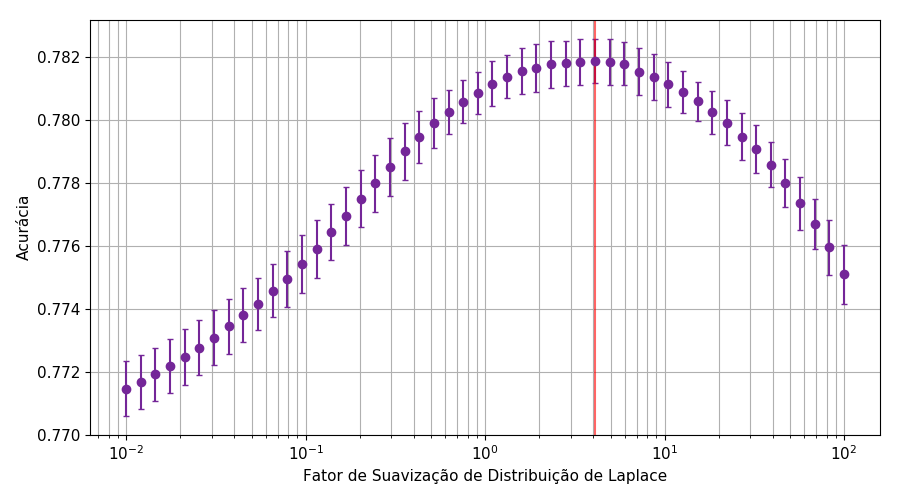
\includegraphics[scale=0.5]{go_nb.png}
    \caption{Seleção do modelo de Naïve Bayes - Etapa 1.}
    \label{fig:go_nb}
    \end{center}
}
\end{center}
\end{figure}

A seleção de modelo formado por \textit{support vector machines} foi feita por processo semelhante ao anterior.
Foram variados o fator de regularização L2, selecionando o modelo de maior percentual de acurácia.
A Figura~\ref{fig:go_svm} apresenta os resultados obtidos, no qual o fator de $6 \times 10^{-6}$ resultou na acurácia
média de 80.0\% sobre o conjunto de validação.
O modelo selecionado apresenta 83,0\% de acurácia no conjunto de testes.

\begin{figure}
\begin{center} {
    \begin{center}
    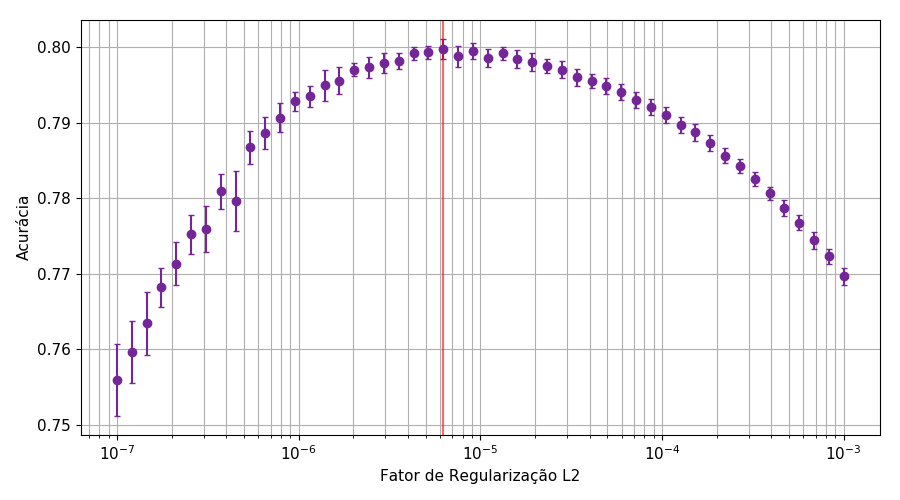
\includegraphics[scale=0.5]{go_svm.png}
    \caption{Seleção do modelo de SVM - Etapa 1.}
    \label{fig:go_svm}
    \end{center}
}
\end{center}
\end{figure}

A tabela~\ref{tab:go_compara} apresenta os resultados obtidos tanto no Sentiment140 quanto pela replicação de
seu método.
Pode se observar que foram atingidos valores próximos a referência, validando assim os pré-processamentos e as
implementações dos algoritmos aplicados.

% Resultados pós calibração
\begin{table}[h]
    \begin{center}
        \begin{tabular}{| l | r | r |}
        \hline
        \textbf{Algoritmo} & \textbf{Original} & \textbf{Replicação} \\ \hline
        Naïve Bayes & 81,3\% & 83,3\% \\ \hline
        SVM &  82,2\% & 83,0\% \\ \hline
        \end{tabular}
        \caption{Comparação de resultados da replicação dos classificadores do Sentiment140.}
        \label{tab:go_compara}
    \end{center}
\end{table}

\section{Segunda Etapa}

A segunda etapa consiste na validação do processo de formação de base de treinamento por supervisão distante.
A aplicação de técnicas de pré-processamento e algoritmos previamente validados neste novo conjunto de dados visa tanto
comparar o processo de elaboração por anotação ruidosa quanto servir como referência para a aplicação de algoritmos de
\textit{deep learning}.
Nesta etapa, os modelos serão avaliados tanto pelo seu desempenho na base de teste disponibilizada por Go
\textit{et al.} quanto quando aplicado na base de testes formada pela coletânea de \textit{tweets} oferecida pelas
conferências SemEval, como descrito na Seção~\ref{sec:data}

Assim como na fase anterior, foram treinados modelos por Naïve Bayes e \textit{support vector machines}.
Neste caso, a seleção dos parâmetros de regularização foi feita de maneira a maximizar a área sob a curva ROC.
As figuras~\ref{fig:nb_selecao} e~\ref{fig:svm_selecao} mostram a resposta dos modelos, respectivamente, Naïve Bayes e
SVM a mudanças nos parâmetros de regularização, as linhas verticais vermelhas apontam os modelos que obtiveram maior
média de área sob a curva ROC dentre os grupos de validação quando aplicada validação cruzada com 10 partições.

\begin{figure}
\begin{center} {
    \begin{center}
    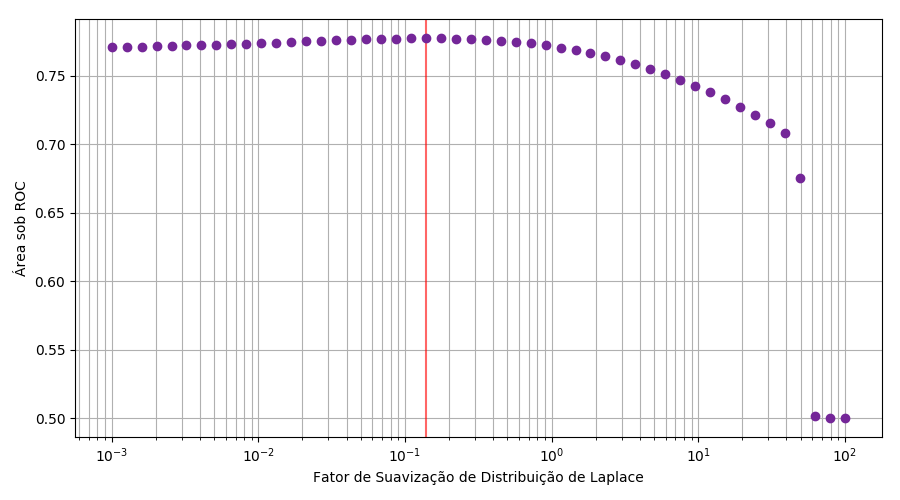
\includegraphics[scale=0.5]{nb_selecao.png}
    \caption{Seleção do modelo de Naïve Bayes - Etapa 2.}
    \label{fig:nb_selecao}
    \end{center}
}
\end{center}
\end{figure}

\begin{figure}
\begin{center} {
    \begin{center}
    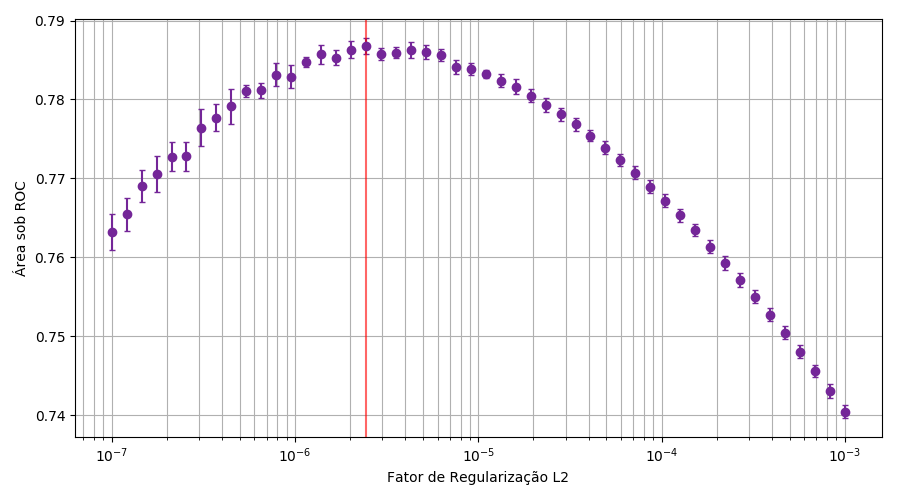
\includegraphics[scale=0.5]{svm_selecao.png}
    \caption{Seleção do modelo de SVM - Etapa 2.}
    \label{fig:svm_selecao}
    \end{center}
}
\end{center}
\end{figure}

Uma vez selecionado os melhores modelos, a Figura~\ref{fig:linear_roc_go} compara a curva ROC que caracteriza a
performance dos modelos treinandos tanto na primeira quanto na segunda etapa sob os dados de testes disponibilizados
por Go \textit{et al.}
A Figura~\ref{fig:linear_roc_semeval} por sua vez apresenta a curva ROC dos modelos quando aplicados nos dados
manualmente anotados coletados do SemEval.

\begin{figure}
\begin{center} {
    \begin{center}
    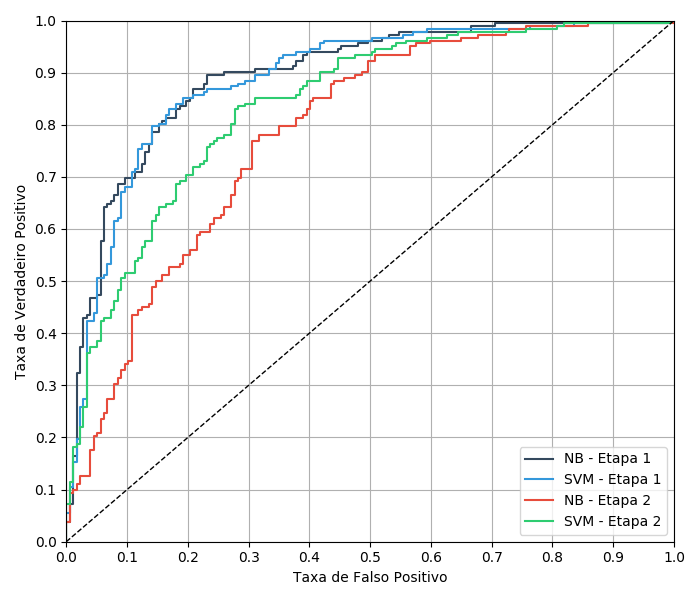
\includegraphics[scale=0.5]{linear_roc_go.png}
    \caption{Curva ROC dos modelos aplicados aos dados de teste do Sentiment140.}
    \label{fig:linear_roc_go}
    \end{center}
}
\end{center}
\end{figure}

\begin{figure}
\begin{center} {
    \begin{center}
    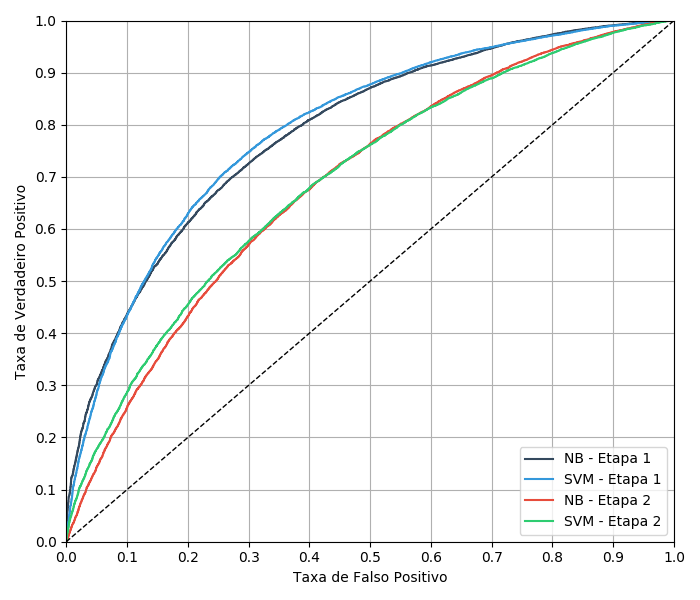
\includegraphics[scale=0.5]{linear_roc_semeval.png}
    \caption{Curva ROC dos modelos aplicados aos dados de teste do SemEval.}
    \label{fig:linear_roc_semeval}
    \end{center}
}
\end{center}
\end{figure}

Observa-se que os modelos modelos treinados pelo conjunto de dados de anotação ruidosa disponibilizados por Go
\textit{et al.} apresentou desempenho consideravelmente melhor nos dois conjuntos de testes.
Desta maneira, se percebe que o processo de anotação dos dados foi mais ruidoso do que o apresentado no Sentiment140.

Uma hipótese a ser feita é que evoluções no idioma e na plataforma durante o intervalo entre a criação de ambas as
bases anotadas por supervisão distante tenha dificultado este processo, visto que a desenvolvida por Go \textit{et al.}
foi coletada em 2009, e a base de treinamento coletada por este trabalho conta com \textit{tweets} de 2017.
Constatou-se, por exemplo, que a base desenvolvida neste trabalho apresentou 1,1 milhões de palavras únicas após o
processo de tokenização, enquanto os dados de treinamento do Sentiment140 contam com 330 mil palavras únicas.
A maior dimensionalidade do problema pode dificultar o processo de treinamento dos algoritmos de aprendizado de máquina.

Outro fator relevante para definição de ruído no processo de anotação é a escolha dos \textit{emoticons}.
Neste trabalho, os \textit{emoticons} mais presentes nos dados foram selecionados para classificação manual, a escolha
de \textit{emoticons} com maior correlação com as classes pode reduzir a diferença entre os resultados de treinamento e
os resultados de teste.
% adicionar desbalanceamento ?

Apesar dos resultados obtidos na base de treinamento anotada para este trabalho serem inferiores aos apresentados pelos
classificadores treinados com a base disponibilizada por Go \textit{et al.}, a técnica de supervisão distante por
\textit{emoticons} para anotação ruidosa de mensagens de redes sociais se mantém como boa alternativa ao processo
custoso de anotação manual.

A Tabela~\ref{tab:linear_perf} apresenta os resultados dos modelos treinados na primeira e na segunda etapas quando
aplicados sob ambos os conjuntos de testes.
O ponto de operação dos modelos foi escolhido de maneira a maximizar o índice SP.
É válido ressaltar que a acurácia é uma métrica inconsistente quando consideras bases de testes com classes
desbalanceadas, como é o caso da base de \textit{tweets} coletados dos SemEval, sendo a área sob a curva ROC, AUC, ou o
índice SP, melhores opções para comparação destes casos.

% AUC -> CalibratedClassifier
% Acurácia, SP -> treshold: ponto de maior SP
\begin{table}[h]
    \begin{center}
        \begin{tabular}{ |l|l|l|r|r|r| }
            \hline
            \textbf{Dados de teste} & \multicolumn{2}{|c|}{\textbf{Modelo}}  & \textbf{Acurácia} & \textbf{AUC} & \textbf{SP} \\ \hline
            \multirow{4}{*}{Sentiment140} & \multirow{2}{*}{Etapa 1} & NB  & 83.3\% & 0.893 & 0.831 \\ \cline{3-6}
                                          &                          & SVM & 83.0\% & 0.887 & 0.830 \\ \cline{2-6}
                                          & \multirow{2}{*}{Etapa 2} & NB  & 73.3\% & 0.785 & 0.732 \\ \cline{3-6}
                                          &                          & SVM & 77,7\% & 0,839 & 0,776 \\ \hline
            \multirow{4}{*}{SemEval}      & \multirow{2}{*}{Etapa 1} & NB  & 70,9\% & 0,786 & 0,713 \\ \cline{3-6}
                                          &                          & SVM & 72,8\% & 0,791 & 0,724 \\ \cline{2-6}
                                          & \multirow{2}{*}{Etapa 2} & NB  & 64,9\% & 0,688 & 0,639 \\ \cline{3-6}
                                          &                          & SVM & 64,2\% & 0,693 & 0,640 \\ \hline
        \end{tabular}
        % FIX
        \caption{Resultados obtidos pelos classificadores.}
        \label{tab:linear_perf}
    \end{center}
\end{table}

\section{Terceira Etapa}
% maximizar roc
% compensar desbalanceamento
